\section{Supplement to Section 7: delayed feedback and robustness}\label{supp:delayed}

This section gives the full text of Section~\ref{M-sec:delayed} (Sections~\ref{supp:std-delayed-law} and~\ref{supp:std-delayed-robust}) and then collects its details and secondary results.

% Moved from Section 7 of the long version (sections/s7_delayed.tex) to keep the article at standard length:
% the full former Section 7, input right after the \section line of Supplement S7.
% Text copied verbatim; only references are adapted (M- = main article; no prefix = Supplementary Material).
% The displayed law eq:comb-law stays in the article; here it is cited with the prefix M-.

\subsection{A delayed term that vanishes on the forced orbit: a case study}\label{supp:std-delayed-law}

Two questions remain for a design that rests on the free voltage: whether a control law can spend the authority on the deviation from the forced orbit alone, and how robust the free voltage and the basin are to errors in the model. The first is answered by a case study of a published delayed term, the second by a Monte Carlo study (Section~\ref{supp:std-delayed-robust}).

The DVF command of Eq.~\eqref{M-eq:dvf} is replaced by the command $u(t)$ of Eq.~\eqref{M-eq:comb-law}, clipped as before, $V=\sat_{\Vmax}(u)$, and studied with $k_d=0$ (DVF\,+\,D). In the Laplace domain $U(s)=-\bigl[s\,K(s)+k_d\,E(s)\bigr]X(s)$ with $K(s)=g_1+g_2E(s)$ and $E(s)=1-e^{-sT}$. The delayed terms vanish on every $T$-periodic motion, since $E(im\omega_T)=0$ at every tooth-passing harmonic, so the forced orbit, its command $b(t)=-g_1\dot x_p(t)$ and the free voltage $u_0$ depend on $g_1$ alone, while a deviation from the orbit meets the full law. Without loop delay $K$ is positive real and the loop passive like DVF \citep{elliott2001feedback}. The law is published: its non-invasiveness is that of Pyragas-type delayed feedback \citep{pyragas1992continuous}, applied to milling by \citet{vandewouw2015ifac} and \citet{vandijk2015ijrnc}; \citet{li2022ijamt} fed back $x(t)-x(t-T)$ to lower the actuator voltage, and delayed feedback has countered regeneration in turning \citep{mancisidor2019mechatronics} and milling \citep{du2022time,du2024ijms}. It is used here to test whether linear margin translates into tolerance of disturbances under a hard clip. The models, the certificate with the delayed terms and the robustness study are detailed in Sections~\ref{supp:mc}--\ref{supp:delayed-robust}.
% src: README §13.2; src/c4_comb.py (docstring, model), src/c4_robust.py (controller); tests/test_c4_comb.py (test_comb_terms_vanish_on_the_settled_cut); paper/notes/novelty.md §1.6

Both families were designed by the authority rule of Eq.~\eqref{M-eq:feas}: $g_1$ is the largest gain up to \SI{3000}{\volt\second\per\metre} whose steady forced command stays within \SI{9}{\volt} up to 0.9 times the design's own linear limit, so that in effect the same gain is compared with and without the delayed term. With $g_2=\SI{2000}{\volt\second\per\metre}$ the linear limit rises by a median factor of 1.78 (1.44--2.10) over the 251 speeds (Fig.~\ref{fig:dlim}a). Much of this rise, however, lies at depths that are not usable: the limit exceeds \SI{32}{\milli\metre}, twice the cutter diameter, at 222 of the 251 speeds, against 71 for DVF, and with the depth capped at \SI{32}{\milli\metre} the median gain falls to 1.31; the cutting tests of \citet{ozsoy2026robust} went up to \SI{10}{\milli\metre}.
% src: results/c4_limits.npz (feas_g1: max |g1 - g1_DVF| = 9.7 V s/m); results/c4_summary.json (limits.feasible: d2000 ratio_to_dvf median 1.78, range 1.44-2.10); verification/paper/revision_runs.json (stored.depth_2D: d2000_above_32mm 222, dvf_above_32mm 71 of 251; median_ratio 1.781, median_ratio_capped_32mm 1.309); verification/targets/experimental_points.csv (tested depths up to 10 mm)

The clipped entries tell a different story (Fig.~\ref{fig:dlim}b). Simulated at 25 speeds with the \SI{9}{\volt} clip, the face-entry limit rises with D by a median factor of 1.72, but the step-entry limit by only 1.03 (0.98--1.27): from \SI{2100}{\rpm} upwards D changes it by at most \SI{1.1}{\milli\metre}, as this limit is set by saturation during the entry, not by damping. The band in which the outcome depends on the entry therefore widens, from a median width of 7.6 to \SI{26}{\milli\metre}. At the same forced command, adding the term with its certificate-optimal $g_2$, which was \SI{500}{\volt\second\per\metre} at every point, to the $g_1$ of the certificate-optimal DVF design widens the simulated basin (worst-phase critical kick) by a median factor of only 1.14 over 22 depth--speed pairs, by about 2 where the DVF certificate almost vanishes, and by 0.96--1.16 below \SI{18}{\milli\metre}; the certified kicks lie below the simulated ones at all 89 points where a kick of up to \SI{3}{\metre\per\second} caused chatter. The term is also fragile: the phase of $E(i\omega)$ alternates between lead and lag between tooth-passing harmonics, and with assumed second modes at 400--\SI{800}{\hertz} the design with $g_2=2000$ tolerates a loop delay of \SI{100}{\micro\second} but not \SI{200}{\micro\second}, against 300 but not \SI{400}{\micro\second} for DVF; a delay \SI{2}{\percent} longer than $T$ makes the term act on the forced orbit and lowers its linear limit to 0.87--0.93 of the nominal value, and with runout its worst command reaches \SI{9}{\volt} at 1.0--\SI{2.4}{\micro\metre}, against 1.1--\SI{4.5}{\micro\metre} for DVF.
% src: results/c4_entry.npz (face 1.45-2.12, median 1.72; step 0.98-1.27, median 1.03; from 2100 rpm +1.08 mm at most; band widths medians 7.56 and 25.88 mm); results/c4_summary.json (validate2: same_g1_over_dvf median 1.14 over 22 pairs; same_g1_near_dvf_limit 1.79-2.59, median 2.00; below 18 mm 0.96-1.16; all_cert_below_td 89/89); results/c4_summary.json (robust.by_rpm: loop delay 300/200/100/100 us for DVF/1000/2000/4000; runout_tolerance_um g2 = 2000 1.03-2.42, DVF 1.12-4.50; tau_us grid 0/50/100/200/300/400; c4_validate2.npz kind same_g1: g2 = 500 at all 25 points; tooth comb eps +2 %: limit 0.87-0.93); paper/figures/figure_numbers.json (fig10)

\begin{figure}[!tbp]
  \centering
  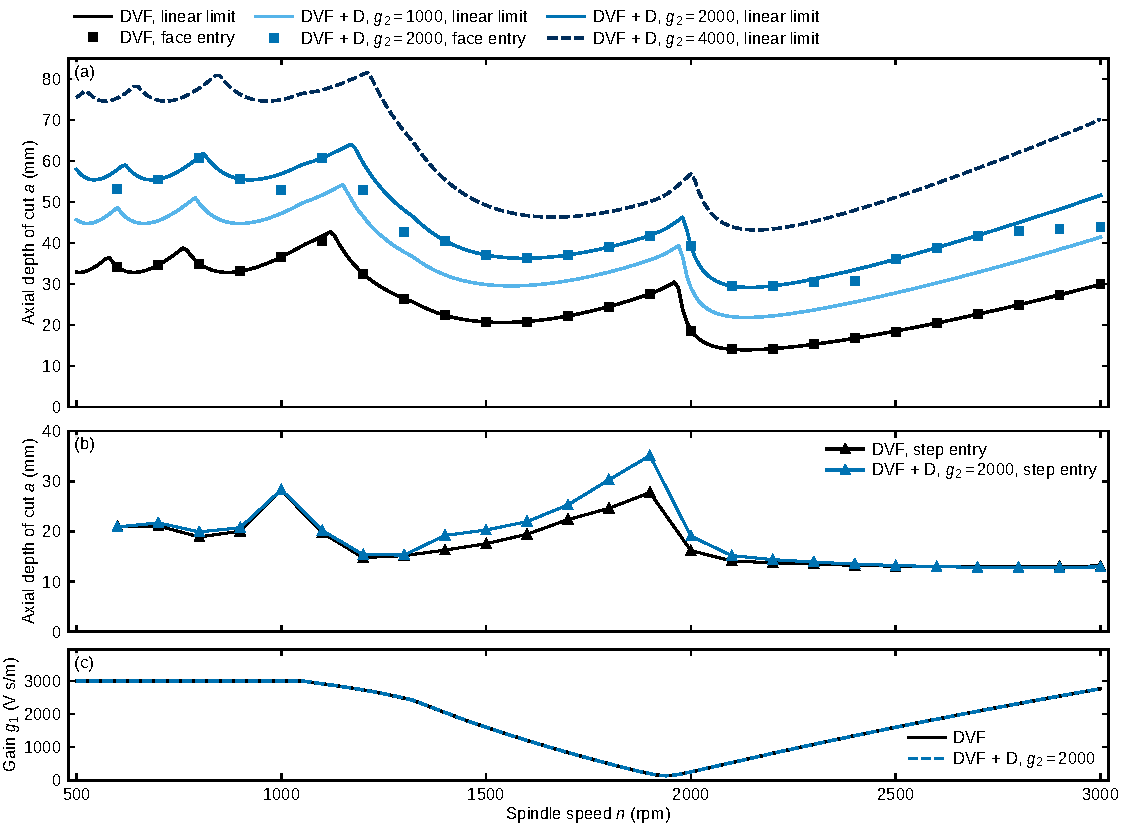
\includegraphics[width=0.86\textwidth]{figures/fig08_delayed_limits.pdf}
  \caption{The delayed term under the same authority rule ($g_1\le\SI{3000}{\volt\second\per\metre}$; steady forced command within \SI{9}{\volt} up to 0.9 of the design's own $\alim$). (a)~Linear limits of DVF and of DVF\,+\,D with $g_2=1000$, 2000 and \SI{4000}{\volt\second\per\metre}; squares: simulated face-entry limits ($\lvert V\rvert\le\SI{9}{\volt}$, 25 speeds) of DVF and of DVF\,+\,D with $g_2=2000$; dash-dotted: $2D=\SI{32}{\milli\metre}$, twice the cutter diameter. (b)~Simulated step-entry limits of the same two designs: the linear margin gained by the delayed term hardly reaches the clipped step entry.}
  \label{fig:dlim}
\end{figure}

The case study thus gives a negative result that matters for design: a law that raises the linear limit by 78\,\% and spends no authority on the forced orbit raises the depth reached by an abrupt entry by 3\,\%, because the entry transient, not the damping of the chatter mode, saturates the actuator. Linear margin is not tolerance of disturbances.

\subsection{Robustness of the residual authority and of the basin}\label{supp:std-delayed-robust}

The residual authority of the nominal design was sampled under errors in the model (Table~\ref{tab:mc}). The cutting coefficients were drawn independently and uniformly within $\pm\SI{10}{\percent}$ of their nominal values (in a second case $\pm\SI{20}{\percent}$), the natural frequency within $\pm\SI{5}{\percent}$, the damping ratio within $\pm\SI{20}{\percent}$, the actuator force constant within $\pm\SI{10}{\percent}$, the eccentric runout within 0--\SI{5}{\micro\metre}, the clip level within 8.1--\SI{9}{\volt} and the loop delay within 0--\SI{300}{\micro\second}; for 4000 samples per case the linear limit and the forced command, the worst over eight phases of the runout, of the $g=1500$ design were computed in closed form at depths fixed as fractions of the nominal $\alim$. At the design depth $0.9\,\alim$ the sampled cut is linearly unstable in 8--\SI{20}{\percent} of the samples, and its forced orbit reaches the clip in up to \SI{9}{\percent}; at $0.98\,\alim$ the two together take 32--\SI{79}{\percent}. Even at half the limit, the forced orbit reaches the clip in 69 and \SI{50}{\percent} of the samples at 2500 and \SI{2870}{\rpm}, where the nominal residual authority is only 1.5 and \SI{3.2}{\volt} at that depth. There the runout dominates (Spearman rank correlation with $u_0$ of $-0.62$ and $-0.83$), whereas near the limit the cutting coefficient, the natural frequency and the actuator constant dominate through the linear limit itself. Widening the range of the cutting coefficients to $\pm\SI{20}{\percent}$ raises the probability of linear instability at $0.9\,\alim$ to 15--\SI{22}{\percent}. In the simulator, with the sampled runout, clip and loop delay, the worst-phase critical kick at $0.9$ of the nominal $\alim$ was found for the first 25 samples at each speed (Section~\ref{supp:mc}). In one or two of them per speed the cut did not settle, being linearly unstable at the sampled parameters or, at \SI{2870}{\rpm}, its forced command exceeding the clip by several volts. In 92 of the other 93 samples the critical kick was 0.39--2.04 times its nominal value (medians 0.81--1.16 over the speeds) and below half of it in three, and in one no kick up to \SI{3}{\metre\per\second} ended in chatter. It followed the margin to the sampled linear limit (rank correlation 0.64--0.90) more closely than the residual authority (0.21--0.43), except at \SI{2870}{\rpm} (0.67 against 0.74), where the runout dominates the latter. Such samples show how the basin moves with the errors but bound nothing: with one or two unsettled samples in 25, the 95\,\% upper confidence bound on that probability is 18--\SI{23}{\percent}.
% src: verification/paper/mc_closed_form.json (levels.pm10/pm20.ranges; n_per_case 4000; speeds.*.fracs.*.p_unstable, p_saturated, u0_stable_median_V, dominant_u0_all, spearman_u0_all: 2500 rpm 0.5 runout -0.62, 2870 rpm 0.5 runout -0.83; nominal.u0_9V); mc_closed_form.py, mc_common.py (caches restored; nominal reproduces stored a_lim and bmax: checks.nominal)
% src (simulated): verification/paper/mc_kick.py/.json (protocol: first 25 samples of the pm10 draw, seed 20261124, 0.9 nominal a_lim, g 1500, phases 0/4/8/12 of 16, face entry, full memory, judged once per revolution); verification/paper/mc_kick_stats.py/.json (speeds.*: unsettled 2/2/1/2, unsettled_reasons linearly unstable at 1090/1420/2500, forced command at the clip at 2870; inf 1/0/0/0; finite 22/23/24/23; all.ratio_min 0.386, ratio_max 2.044, ratio_median_range 0.805-1.158; below_half_nominal 0/2/1/0; spearman_kick_vs_alim_margin 0.879/0.904/0.641/0.673; spearman_kick_vs_u0_worst_psi 0.209/0.416/0.432/0.735; cp95_upper_unsettled 0.231/0.231/0.176/0.231)

\begin{table}[!tbp]
  \centering
  \caption{Monte Carlo of the residual authority $u_0=V_{\mathrm{clip}}-\bmax$ of the $g=\SI{1500}{\volt\second\per\metre}$ design (closed-form zero-order model; forced command the worst over eight runout phases; 4000 samples per case; depth fixed at a fraction of the nominal $\alim$; parameter ranges in the text). $\pm\SI{10}{\percent}$, $\pm\SI{20}{\percent}$: range of the cutting coefficients. $u_0$ in volts; median over the linearly stable samples. Unstable: linearly unstable samples; clip: stable samples whose forced orbit reaches the clip ($u_0\le0$); both in per cent of the samples. These are frequencies over an assumed distribution, not a guarantee.}
  \label{tab:mc}
  \small
  \begin{tabular}{@{}rcccccrr@{}}
    \toprule
    Speed & $a/\alim$ & Nominal & \multicolumn{3}{c}{$\pm\SI{10}{\percent}$} & \multicolumn{2}{c}{$\pm\SI{20}{\percent}$}\\
    \cmidrule(lr){4-6}\cmidrule(l){7-8}
    (rpm) & & $u_0$ & median $u_0$ & unstable & clip & unstable & clip\\
    \midrule
    1090 & 0.5 & 4.72 & 3.69 & 0 & 0 & 0 & 0\\
     & 0.7 & 4.65 & 3.71 & $<1$ & 0 & 1 & 0\\
     & 0.9 & 4.69 & 3.96 & 20 & 0 & 20 & 0\\
     & 0.98 & 4.01 & 3.20 & 32 & 0 & 31 & 0\\
    \addlinespace
    1420 & 0.5 & 2.68 & 1.80 & 0 & $<1$ & 0 & 2\\
     & 0.7 & 8.72 & 7.79 & 0 & 0 & 0 & 0\\
     & 0.9 & 2.91 & 1.98 & 12 & $<1$ & 22 & 1\\
     & 0.98 & 1.79 & 1.21 & 48 & 2 & 49 & 2\\
    \addlinespace
    2500 & 0.5 & 1.49 & -0.65 & 0 & 69 & 0 & 65\\
     & 0.7 & 7.76 & 6.14 & 0 & 0 & $<1$ & 0\\
     & 0.9 & 2.79 & 1.58 & 11 & 4 & 15 & 8\\
     & 0.98 & 1.13 & -0.63 & 31 & 48 & 33 & 39\\
    \addlinespace
    2870 & 0.5 & 3.24 & 0.01 & 0 & 50 & 0 & 49\\
     & 0.7 & 5.99 & 2.29 & 0 & 19 & 0 & 19\\
     & 0.9 & 6.74 & 4.12 & 8 & 9 & 15 & 7\\
     & 0.98 & 5.04 & 3.30 & 34 & 3 & 39 & 2\\
    \bottomrule
  \end{tabular}
\end{table}
% src: verification/paper/mc_closed_form.json (nominal.<rpm>.u0_9V; levels.pm10/pm20.speeds.<rpm>.fracs.<frac>: u0_stable_median_V, p_unstable, p_saturated)

The clip level itself is a design choice (Section~\ref{supp:std-model-act}). Lowering it from 9 to \SI{8.1}{\volt}, which kept the peak actuator force at \SI{26.6}{\newton} in the deepest stable step entry at \SI{2500}{\rpm}, reduces the residual authority at $0.9\,\alim$ to 0.68--0.87 of its value and the worst-phase critical kick there to 0.76--0.88 of its value at the four speeds, close to the ratios of 0.78--0.89 that the describing function of Eq.~\eqref{M-eq:dfbasin} predicts; at \SI{2500}{\rpm} the forced command exceeds \SI{8.1}{\volt} already at 0.27--$0.46\,\alim$, by up to \SI{0.47}{\volt}, and again near $\alim$, so that with this clip the forced orbit itself is clipped there and the basin closes before the limit. A force limit enforced by lowering the clip is thus paid for in tolerated disturbance.
% src: verification/paper/protocol_clip_level.json (summary: ratio_of_minima 0.850/0.763/0.763/0.878 at 1090/1420/2500/2870 rpm, 0.9 a_lim, phases 0, 4, 8, 12; df_ratio_prediction 0.845/0.801/0.778/0.892; free_voltage_ratio_at_0p9alim 0.808/0.690/0.677/0.866; free_voltage_ratio_at_alim at 2500 rpm -0.038); verification/paper/support_runs.json (26.6 N at 8.1 V, deepest stable step entry at 2500 rpm, g = 1500); verification/paper/clip81_forced_command.py/.json (2500 rpm: intervals_above_clip_frac 0.27-0.46 and 0.9975-1, max_V 8.570 at 0.35 a_lim, V_at_a_lim 8.13; none at 1090, 1420, 2870 rpm)


\subsection{Monte Carlo of the residual authority}\label{supp:mc}

\paragraph{Closed form} The cutting coefficients $K_{tc}$ and $K_{rc}$ were drawn independently and uniformly within $\pm\SI{10}{\percent}$ (and, with the same uniform draws, within $\pm\SI{20}{\percent}$) of their nominal values, the natural frequency within $\pm\SI{5}{\percent}$ with the stiffness fixed, the damping ratio within $\pm\SI{20}{\percent}$, the actuator constant $K_a$ within $\pm\SI{10}{\percent}$, the eccentric runout within 0--\SI{5}{\micro\metre}, the clip within 8.1--\SI{9}{\volt} and the loop delay within 0--\SI{300}{\micro\second}, 4000 samples per case. For each sample the linear limit of the delayed DVF loop of the $g=1500$ design was computed in the zero-order model, and the forced command at the fixed depth as the worst over eight runout phases; with 32 phases the command rises by at most \SI{15}{\milli\volt}. The nominal sample reproduces the stored limits, free voltages and runout tolerances. With the runout set to zero, the probability that the forced orbit reaches the clip at half the limit falls from 69 to \SI{33}{\percent} at \SI{2500}{\rpm} and from 50 to \SI{0.03}{\percent} at \SI{2870}{\rpm}.
% src: verification/paper/mc_closed_form.py, mc_common.py (ranges, seed, caches restored), mc_closed_form.json (levels.pm10.speeds.2500.fracs.0.5.no_runout.p_saturated 0.328, 2870 0.00025; checks.nominal reproduces the stored a_lim, free voltage and runout tolerance; n_psi_8_vs_32 max_underestimate_V 0.0152)

\paragraph{Simulated critical kick} For the first 25 samples of the $\pm\SI{10}{\percent}$ draw, at the four speeds and at 0.9 of the nominal $\alim$ ($g=\SI{1500}{\volt\second\per\metre}$), the cut was simulated with the sampled parameters, its own runout amplitude and phase, clip and loop delay, the full surface memory and a face entry, and kicked at revolution 100 at four phases a quarter of a tooth period apart, with the kick search of Section~\ref{M-sec:bistab-prot}; a phase was abandoned as soon as its critical kick was proven larger than the smallest so far, which leaves the minimum unchanged. With runout the settled orbit is periodic in the spindle revolution, which the tooth-period classifier would call chatter, so the runs were judged once per revolution with the same thresholds; with the tooth-period classifier the nominal runs reproduce the stored critical kicks exactly. A sampled delay shorter than one time step of the simulator (41--\SI{107}{\micro\second}) was simulated as zero or one step, and the closed-form values of the sample were recomputed with the delay simulated. Table~\ref{tab:mc-kick} gives the results. Seven samples did not settle: five that are linearly unstable at the sampled parameters, and the two at \SI{2870}{\rpm} whose forced command exceeds the sampled clip by 2.9 and \SI{14.5}{\volt}. Two samples that the closed form calls marginally unstable (by 0.5 and \SI{0.3}{\percent} in depth), and two at \SI{2500}{\rpm} whose forced command exceeds the sampled clip by up to \SI{0.35}{\volt}, settled nonetheless and have finite critical kicks.

\begin{table}[!tbp]
\centering
\caption{Simulated worst-phase critical kick (four phases) under the sampled errors of Table~\ref{tab:mc}, 25 samples per speed, $a=0.9\,\alim$ (nominal), $g=\SI{1500}{\volt\second\per\metre}$. Not settled: chatter before the kick. Ratio: critical kick over its nominal value, over the samples with a finite critical kick. $\rho_s$: Spearman rank correlation of the critical kick with the margin $\alim-a$ of the sample and with its residual authority $u_0$ (worst runout phase).}
\label{tab:mc-kick}
\small
\setlength{\tabcolsep}{4pt}
\begin{tabular}{@{}rccccccc@{}}
\toprule
Speed & Nominal & Not & No chatter & Ratio, median & Below & \multicolumn{2}{c}{$\rho_s$ with}\\
\cmidrule(l){7-8}
(rpm) & (\si{\milli\metre\per\second}) & settled & to \SI{3}{\metre\per\second} & (range) & half & $\alim-a$ & $u_0$\\
\midrule
1090 & 15.1 & 2 & 1 & 1.16 (0.62--2.04) & 0 & 0.88 & 0.21\\
1420 & 12.9 & 2 & 0 & 0.81 (0.39--1.83) & 2 & 0.90 & 0.42\\
2500 & 7.3  & 1 & 0 & 0.92 (0.48--1.79) & 1 & 0.64 & 0.43\\
2870 & 11.6 & 2 & 0 & 0.81 (0.51--1.19) & 0 & 0.67 & 0.74\\
\bottomrule
\end{tabular}
\end{table}
% src: verification/paper/mc_kick.py/.json (protocol, nominal.*.worst4_rev_mmps 15.058/12.939/7.288/11.611, worst4_tooth equal; samples.*.tau_sim; cf); verification/paper/mc_kick_stats.py/.json (speeds.*: unsettled 2/2/1/2, inf 1/0/0/0, ratio_median 1.158/0.814/0.917/0.805, ratio_min/max 0.621-2.044, 0.386-1.834, 0.484-1.795, 0.505-1.189, below_half_nominal 0/2/1/0, spearman_kick_vs_alim_margin 0.879/0.904/0.641/0.673, spearman_kick_vs_u0_worst_psi 0.209/0.416/0.432/0.735; cf_unstable_but_settled: sample 11 at 1090 rpm, a_lim 18.80 against 18.89 mm, sample 14 at 1420 rpm, 15.95 against 16.00 mm; mc_kick.json samples: 2870 rpm samples 0 and 19 unsettled with cf.u0_worst_psi_V -2.91 and -14.46; 2500 rpm samples 13 and 17 settled with u0_worst_psi_V -0.35, pre_kick_clipped true)

\subsection{The law, its properties and prior work}\label{supp:delayed-prior}

In the notation of Section~\ref{M-sec:delayed-law}, $K(s)=g_1+g_2E(s)$ and $E(s)=1-e^{-sT}$; the law with $g_2=0$ and $k_d\neq0$ is denoted DVF\,+\,P.

\emph{(ii)~DVF\,+\,D is passive only without loop delay.} For $g_1,g_2\ge0$, $\operatorname{Re}K(s)\ge g_1$ in $\operatorname{Re}s\ge0$, so $K$ is positive real and, with an ideal collocated actuator and no loop delay, the velocity loop is passive like DVF \citep{elliott2001feedback}; $\lvert K(i\omega)\rvert$ lies between $g_1$ at the harmonics and $g_1+2g_2$ halfway between them. With a loop delay $\tau$ the controller becomes $e^{-s\tau}K(s)$, and the phase of $E(i\omega)$, which falls from $+\ang{90}$ to $-\ang{90}$ between consecutive harmonics, adds to the lag of the delay in the upper half of each interval (Section~\ref{M-sec:delayed-robust}).

\emph{(iii)~$k_d$ must be negative.} As $\overline{aH}<0$ [Eq.~\eqref{M-eq:aHmean}] and $G_a\approx K_a$ at the chatter frequency, $k_d=\SI{-e5}{\volt\per\metre}$ adds about \SI{3e5}{\newton\per\metre} to the negative coefficient of $x-x(t-T)$, as much as $\lvert\overline{aH}\rvert$ at $a=\SI{1}{\milli\metre}$, and so offsets about \SI{1}{\milli\metre} of depth.
% src: README §13.2; src/c4_comb.py (docstring, model), src/c4_robust.py (controller); tests/test_c4_comb.py (test_comb_terms_vanish_on_the_settled_cut; test_negative_kd_opposes_regeneration: +0.98 mm for kd = -1e5 V/m at 2500 rpm, g1 = 1500); N_t K_tc |alpha_yy|/(4 pi) x 1 mm = 3.0008e5 N/m from src/params.py; |G_a|/K_a = 1.004 at 129.3 Hz (Section 2.1)

The law is published. Its non-invasiveness on the periodic orbit is that of Pyragas-type delayed feedback \citep{pyragas1992continuous}, which \citet{vandewouw2015ifac} and \citet{vandijk2015ijrnc} applied to high-speed milling, the latter with fixed-structure delayed output feedback that vanishes on the periodic solution and with the actuator forces as a design criterion. \citet{li2022ijamt} fed back $x(t)-x(t-T)$ through a PD law to lower the actuator voltage, delayed feedback has countered the regenerative effect in turning \citep{mancisidor2019mechatronics} and milling \citep{du2022time}, and \citet{du2024ijms} combined it with robust control and reported control voltages 11--\SI{25}{\percent} below those of robust control alone, the same authority argument. What is added here is the analysis under a hard \SI{9}{\volt} clip: the authority budget left by the forced orbit, certified inner estimates of the basin with the delayed terms in the sector argument, their check in the simulator, and the robustness limits of the idealised model.
% src: README §13.2 (prior work; 11-25 % for Du et al. 2024); paper/notes/novelty.md §1.6 (descriptions from abstracts; the full text of vandewouw2015ifac was not checked)

\subsection{Models, certificate and simulator}\label{supp:delayed-model}

\paragraph{Certificate}
The averaged collocation model~\eqref{M-eq:coll} keeps its form, with the DVF row $k^\top=-g\,e_2^\top$ replaced by
\begin{equation*}
  \begin{gathered}
    k^\top=-(g_1+g_2)\,e_2^\top+g_2\,d_N^\top-k_d\,\bigl(e_1-e_{4+N}\bigr)^\top,\\
    d_N^\top\xi=\frac2T\Bigl[(D_N)_{N0}\,\tilde x+\sum_{l=1}^{N}(D_N)_{Nl}\,\tilde x(t+\vartheta_l)\Bigr],
  \end{gathered}
\end{equation*}
where $e_{4+N}^\top\xi=\tilde x(t-T)$ and $d_N^\top\xi$, the derivative of the Chebyshev interpolant of the history at $\vartheta=-T$ (Section~\ref{app:lmi}), stands for $\dot{\tilde x}(t-T)$. As $b(t)$ depends on $g_1$ only, $\bar b$, the sector condition~\eqref{M-eq:sector}, the LMIs \eqref{M-eq:lmi-dec}--\eqref{M-eq:lmi-size} and the check of Section~\ref{M-sec:cert-check} apply unchanged. A velocity kick $\Delta v$, however, leaves a kink in the history that the interpolant smooths, and the delayed command of the model then departs from that of the delay equation by about half of $g_2\Delta v$ in each of the first two tooth periods (DVF: less than \SI{1}{\percent} of $g\Delta v$); the certificate therefore rests more on the simulator check (Section~\ref{supp:delayed-valid}) than in Section~\ref{M-sec:certificates}.
% src: src/c4_comb.py (model, certify_kick; docstring: 0.45-0.5 and 0.5-0.65 g2 per m/s of kick); tests/test_c4_comb.py (test_comb_model_without_comb_is_the_c2_model, test_comb_row_vanishes_on_a_tooth_periodic_state, test_comb_limit_converges_in_the_nodes: limit moves < 1e-4 with 1.6x and 2.4x the nodes at 2500 rpm); README §13.3

\paragraph{Simulator and closed form}
The simulator of Section~\ref{app:simulator} was extended by $g_2$, $k_d$, a comb delay $T_c$ in place of $T$, eccentric runout of the teeth and a loop delay $\tau$. The robustness study uses the averaged model in the frequency domain, with the characteristic function
\begin{equation}\label{eq:comb-char}
  \begin{aligned}
    \Delta(s)&=1-G(s)\Bigl[\overline{aH}\,E(s)-G_a(s)\,e^{-s\tau}\bigl(s\,[g_1+g_2E_c(s)]+k_d\,E_c(s)\bigr)\Bigr],\\
    E_c(s)&=1-e^{-sT_c},
  \end{aligned}
\end{equation}
where $G$ may include an assumed second mode; with $\tau=0$, $T_c=T$ and one mode, $\Delta=0$ is the characteristic equation of the averaged delay equation. Its limits agree with those of the collocation model and of the simulator (Supplementary Material).
% src: README §13.3; src/tdsim.c (COMB build); src/c4_robust.py (delta, unstable_zeros); tests/test_c4_comb.py (test_closed_form_limit_is_the_collocated_limit, 4 cases, rel 2e-4); results/c4_robust.npz and c4_summary.json (robust.td_limit_ratio 1.0025-1.0148, 7 cases)

\subsection{A fair baseline and the linear limit}\label{supp:delayed-limit}

The bound $g\le\SI{1500}{\volt\second\per\metre}$ of Sections~\ref{M-sec:feasibility}--\ref{M-sec:certificates} is a choice of this study, not a property of the actuator, and a comparison at that bound inflates the benefit: added to those gains, $g_2=\SI{2000}{\volt\second\per\metre}$ doubles the linear limit (median ratio 2.0). Both families were therefore designed by the rule of Eq.~\eqref{M-eq:feas}: $g_1$ is the largest gain up to \SI{3000}{\volt\second\per\metre} whose steady forced command stays within \SI{9}{\volt} up to 0.9 times the design's own linear limit. For DVF this is the map with $g_{\max}=3000$ of Section~\ref{M-sec:feas-res}, limited by authority at 195 of the 251 speeds and by the bound at the other 56. Adding $g_2$ or $k_d$ hardly changes $g_1$ (Supplementary Material), so in effect the same gain is compared with and without the delayed term.
% src: results/c4_limits.npz (a_lim at the C1/C2 gain + g2 = 2000: median ratio 2.005; feas_g1: DVF below 3000 at 195 speeds, 1060-3000 rpm; max |g1 - g1_DVF| = 9.7 V s/m, 0.35 %); results/c4_summary.json (limits); src/c4_comb.py (a_lim_ctrl, feasible_g1); tests/test_c4_comb.py (test_feasible_dvf_gain_is_the_feasibility_optimum); README §13.4

With $g_2=2000$ the limit rises by a median factor of 1.78 (1.44--2.10; Table~\ref{tab:dlim}, Fig.~\ref{fig:dlim}a). The rise persists where DVF sits on the bound: with the bound lifted to \SI{20000}{\volt\second\per\metre} for both families at those 56 speeds, DVF\,+\,D still reaches a median 1.47 times the DVF limit, so the D term adds linear margin rather than only redistributing authority. Much of the gain, however, lies at large depths: with $g_2=2000$ the limit exceeds \SI{32}{\milli\metre}, twice the cutter diameter, at 222 of the 251 speeds, against 71 for DVF, and with the usable depth capped at \SI{32}{\milli\metre} the median gain falls from 1.78 to 1.31; the cutting tests of \citet{ozsoy2026robust} went up to \SI{10}{\milli\metre}. The P term shifts the limit by a nearly constant amount, about \SI{1}{\milli\metre} per \SI{-e5}{\volt\per\metre} of $k_d$, as (iii) predicts (Supplementary Material).
% src: results/c4_summary.json (limits.feasible; limits.uncapped: 56 speeds, d2000/DVF 1.31-1.68, median 1.47); results/c4_limits.npz (feas_a_lim differences, recomputed: p3e5 - dvf 2.89-3.02 mm, p1e6 - dvf 9.66-9.93 mm); README §13.4, §13.5
% src (depth qualifier): verification/paper/revision_runs.json (stored.depth_2D: d2000_above_32mm 222, dvf_above_32mm 71 of 251 speeds; median_ratio 1.781, median_ratio_capped_32mm 1.309), recomputed from results/c4_limits.npz (feas_a_lim, feas_names); cutter diameter 16 mm (Table 1); verification/targets/experimental_points.csv (tested depths up to 10 mm)

\begin{table}[!htbp]
  \centering
  \caption{Linear stability limit over 251 speeds (\SIrange{500}{3000}{\rpm}) under the same authority rule [Eq.~\eqref{M-eq:feas} with the design's own $\alim$, $g_1\le\SI{3000}{\volt\second\per\metre}$]; $g_2$ in \si{\volt\second\per\metre}. Ratio to the DVF limit at the same speed: median (range) over all speeds; last column: median over the 195 speeds where the DVF gain is limited by authority / over the 56 where it sits on the bound. The DVF\,+\,P designs are given in the Supplementary Material.}
  \label{tab:dlim}
  \small
  \begin{tabular}{@{}lccc@{}}
    \toprule
    Design & $\alim$ (\si{\milli\metre}) & Ratio to DVF & Median ratio\\
     & & median (range) & authority / bound\\
    \midrule
    DVF & 14.0--42.8 & 1 & --\\
    DVF\,+\,D, $g_2=1000$ & 21.9--54.3 & 1.43 (1.23--1.57) & 1.43 / 1.34\\
    DVF\,+\,D, $g_2=2000$ & 29.2--64.1 & 1.78 (1.44--2.10) & 1.81 / 1.64\\
    DVF\,+\,D, $g_2=4000$ & 43.2--81.6 & 2.40 (1.75--3.15) & 2.50 / 2.20\\
    \bottomrule
  \end{tabular}
\end{table}
% src: results/c4_summary.json (limits.feasible: a_lim_mm, ratio_to_dvf, ratio_authority_limited, ratio_gain_bounded); results/c4_limits.npz; README §13.5



\subsection{Entries in the simulator}\label{supp:delayed-entry}

Step and face entries (Section~\ref{M-sec:bistab-prot}) were simulated with the \SI{9}{\volt} clip at 25 speeds (\SIrange{600}{3000}{\rpm}) for DVF and for DVF\,+\,D with $g_2=2000$ (Fig.~\ref{fig:dlim}a,b). With D the face-entry limit is 1.45--2.12 times higher (median 1.72) and reaches the new linear limit at 16 of the 25 speeds (0.85--$0.98\alim$ at the others). The step-entry limit changes little: the ratio is 0.98--1.27 (median 1.03). From \SI{2100}{\rpm} upwards D changes it by at most \SI{1.1}{\milli\metre}, as this limit is set by saturation during the entry, not by damping; only at \SIrange{1400}{2000}{\rpm}, where the step entry approaches the linear limit, does D raise it markedly (1.13--1.27 times).
% src: results/c4_entry.npz (designs feas_dvf, feas_d2000: a_entry, a_lim, g1; per-speed ratios: face 1.45-2.12, median 1.72; face entry with D at a_lim at 16 speeds, 0.85-0.98 a_lim at nine; step 0.98-1.27, median 1.03; 1.13-1.27 at 1400-2000 rpm, 1.008 at 1300 rpm, recomputed; from 2100 rpm +1.08 mm at most, -0.21 mm at most at 2700-3000 rpm); README §13.6

The band between the step-entry and the linear limit, in which the outcome depends on the entry, therefore widens: the median ratio of the two limits falls from 0.70 for DVF to 0.39 with D, and the median width of the band grows from 7.6 to \SI{26}{\milli\metre}. Most of the depth gained needs a gentle entry.
% src: results/c4_entry.npz (step/a_lim medians 0.704 and 0.390; a_lim - step medians 7.56 and 25.88 mm); README §13.6

\subsection{Certified gain map}\label{supp:delayed-map}

The certified kick $\beta$ [Eq.~\eqref{M-eq:lmi-size} with $e=e_2$] was computed at the four speeds of Section~\ref{M-sec:bistab-basin} and 17 depths (2--\SI{34}{\milli\metre}) for 20 delayed pairs, $g_1\in\{500,1000,1500,2000,3000\}$ and $g_2\in\{500,1000,2000,4000\}$\,\si{\volt\second\per\metre}, and for DVF at 26 gains (500--\SI{3000}{\volt\second\per\metre} in steps of 100), so that DVF has no fewer candidates. Table~\ref{tab:dgap} gives the depth up to which every grid depth is certified with a kick of at least $\beta_{\mathrm{th}}$. At $\beta_{\mathrm{th}}=\SI{1}{\milli\metre\per\second}$ the delayed term covers the whole grid at all four speeds, against 16--\SI{34}{\milli\metre} for DVF, and the advantage narrows as $\beta_{\mathrm{th}}$ grows. These thresholds are small: as equivalent displacements $\beta_{\mathrm{th}}/\omega_n$, 1, 2 and \SI{4}{\milli\metre\per\second} are 1.2, 2.5 and \SI{4.9}{\micro\metre}, and a kick of \SI{1}{\milli\metre\per\second} carries only 0.5--\SI{1.3}{\percent} of the cutting impulse of one tooth period [Eq.~\eqref{M-eq:impulse}] at \SI{16}{\milli\metre}, whereas kicks of 2.4--\SI{10.8}{\percent} tip the clipped DVF cut into chatter near its limit (Section~\ref{M-sec:bistab-basin}).
% src: src/c4_comb.py (GM_RPM, GM_DEPTH, GM_G1, GM_G2, GM_G1_DVF; run_gainmap); results/c4_gainmap.npz; results/c4_summary.json (gainmap.by_rpm.certified_without_gap_mm); results/c3_summary.json (errata.c4_gainmap: size_factor 0.593-1, table unchanged); impulse shares recomputed from Eq. (impulse) with src/params.py: 0.48-1.25 % at 16 mm; beta_th / omega_n with omega_n = 2 pi x 129.3 rad/s (src/params.py FN): 1.231, 2.462, 4.924 um; README §13.7, §14.9

The certificate picks the smallest gain with enough linear margin: with D it keeps $g_1$ at 500--1000 at most depths and raises $g_2$ to 2000--4000 where the DVF certificate is small or absent (Fig.~\ref{fig:dbasin}). Where both families are certified, the best delayed certificate exceeds the best DVF one by a median factor of only 1.05--1.08 per speed.
% src: results/c4_gainmap.npz (maximising designs per speed and depth: delayed optimum g1 = 500-1000 except at 24-26 mm and at 2870 rpm, 12 mm; g2 >= 2000 only where the best DVF certificate is 0-3.5 mm/s, recomputed); results/c4_summary.json (gainmap.by_rpm.comb_over_dvf medians 1.08, 1.05, 1.07, 1.06); README §13.7

\begin{table}[!htbp]
  \centering
  \caption{Certified depth without a gap (\si{\milli\metre}): the largest depth of the grid (2--\SI{34}{\milli\metre}, step \SI{2}{\milli\metre}) up to which every grid depth is certified with a kick of at least $\beta_{\mathrm{th}}$ by the best candidate design ($\lvert V\rvert\le\SI{9}{\volt}$; averaged collocation model, in which the delayed velocity of DVF\,+\,D is the derivative of the history interpolant, Section~\ref{supp:delayed-model}; certificates rescaled to the rigorous bound $\bar b$). $\ge34$: the whole grid.}
  \label{tab:dgap}
  \small
  \begin{tabular}{@{}llcccc@{}}
    \toprule
    $\beta_{\mathrm{th}}$ (\si{\milli\metre\per\second}) & Candidates & \SI{1090}{\rpm} & \SI{1420}{\rpm} & \SI{2500}{\rpm} & \SI{2870}{\rpm}\\
    \midrule
    1 & DVF, 26 gains & $\ge34$ & 18 & 16 & 28\\
      & DVF\,+\,D, 20 pairs & $\ge34$ & $\ge34$ & $\ge34$ & $\ge34$\\
      & DVF\,+\,D, $g_2\le2000$ & $\ge34$ & 30 & 28 & $\ge34$\\
    2 & DVF, 26 gains & 32 & 16 & 16 & 16\\
      & DVF\,+\,D, 20 pairs & $\ge34$ & 30 & 28 & $\ge34$\\
    4 & DVF, 26 gains & 26 & 16 & 14 & 14\\
      & DVF\,+\,D, 20 pairs & 28 & 26 & 16 & 18\\
    \bottomrule
  \end{tabular}
\end{table}
% src: results/c4_summary.json (gainmap.by_rpm.certified_without_gap_mm: dvf_*, comb_*, comb_g2le2000_1); results/c3_summary.json (errata.c4_gainmap.certified_without_gap_mm: unchanged by the correction); README §13.7 (table), §14.9

\subsection{Validation of the delayed designs in the simulator}\label{supp:delayed-valid2}

At the four speeds and 6--\SI{34}{\milli\metre}, 100 design points were simulated: the DVF designs with the largest certified kick over 26 and over five gains, the delayed design with the largest certified kick (the \emph{map design}) and the \emph{same-$g_1$ design}, which adds to the $g_1$ of the 26-gain DVF optimum the $g_2$ that maximises its certificate. The same-$g_1$ design has the forced orbit and the authority budget of that DVF, so any change of its basin is due to the delayed term alone. At each point the critical kick $\Delta v^*$ (worst of 16 phases), the certified kick and the critical kick of the collocation model were computed (Supplementary Material).
% src: src/c4_comb.py (VAL_DEPTH, VAL2_DEEP, best_gains, _same_g1, run_validate, run_validate2); results/c4_validate.npz (22 dvf, 24 comb), results/c4_validate2.npz (21 dvf_fine, 25 same_g1, 8 comb); README §13.8

No unkicked cut chattered. The certified kick lies below $\Delta v^*$ at all 89 points where a kick of up to \SI{3}{\metre\per\second} ended in chatter, by factors of 1.6--7.3 (median 2.3), and below the critical kick of the collocation model at all 97 points where that kick is finite. Despite the error in its delayed velocity, the collocation model reproduces $\Delta v^*$ no worse than for DVF: its critical kick is 0.80--1.01 (median 0.98) times $\Delta v^*$ for the map designs and 0.79--1.00 (median 0.96) for the same-$g_1$ designs, against 0.66--1.02 for DVF.
% src: results/c4_validate.npz, results/c4_validate2.npz (unsettled 0; td_min infinite at 11 points; model_kick infinite at 3); results/c4_summary.json (validate2: all_cert_below_td 89/89, all_cert_below_model 97/97); results/c3_summary.json (errata.c4_validate: corrected 1.60-7.32, median 2.29); README §13.8, §14.9
% src (model to simulated critical kick): results/c4_validate.npz and c4_validate2.npz recomputed: comb 29 points 0.80-1.01 (median 0.98), same_g1 22 points 0.79-1.00 (median 0.96), dvf and dvf_fine 38 points 0.66-1.02

The basins were compared at the 22 depth--speed pairs where both families have a finite $\Delta v^*$ (Fig.~\ref{fig:dbasin}). At the same forced command, the same-$g_1$ design raises $\Delta v^*$ by a median factor of 1.14 over all 22 pairs (larger at 19), by 1.45 over the 13 pairs at \SI{18}{\milli\metre} and deeper, and by 2.00 (1.79--2.59) over the six pairs, all at 18--\SI{34}{\milli\metre}, where the DVF certificate is at most \SI{2.1}{\milli\metre\per\second}; this threshold is descriptive and has no physical meaning. Below \SI{18}{\milli\metre} the basin hardly widens (0.96--1.16). The delayed term thus widens the basin through its linear margin, not by freeing authority. The certificate chose $g_2=500$, the smallest of the grid, for every same-$g_1$ design, and no other $g_2$ was simulated.
% src: results/c4_summary.json (validate2: same_g1_over_dvf 0.96-2.59, median 1.14, 19/22; same_g1_deep: 13 pairs, 1.06-2.59, median 1.45; same_g1_near_dvf_limit: DVF certified kick <= 2.1 mm/s, 6 pairs: 1420 rpm at 18 and 22 mm, 2500 rpm at 22 mm, 2870 rpm at 18 and 22 mm, 1090 rpm at 34 mm; 1.79-2.59, median 2.00; below 18 mm 0.96-1.16, recomputed from pairs_mmps); results/c4_validate2.npz (same_g1: g2 = 500 at all 25 points); README §13.8

The map design, which also frees authority, is ahead of the 26-gain DVF at 18 of the 22 pairs (median ratio 1.11), but against the better of the two DVF designs at only 13 (median 1.04). The gains that maximise the certificate are not those that maximise the basin: its preference for a small $g_1$ can narrow the basin at shallow depths (Supplementary Material).
% src: results/c4_summary.json (validate2: comb_over_dvf 0.82-3.02, median 1.11, 18/22; comb_over_better_dvf 0.81-3.02, median 1.04, 13/22; pairs_mmps); README §13.8

\begin{figure}[!htbp]
  \centering
  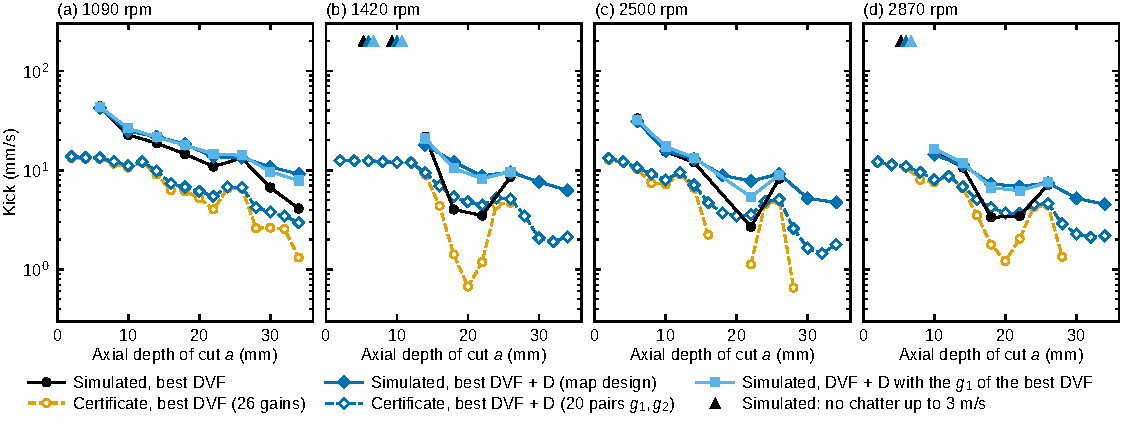
\includegraphics[width=\textwidth]{figures/fig09_delayed_basin.pdf}
  \caption{Certified and simulated kicks with the delayed term at (a)~1090, (b)~1420, (c)~2500 and (d)~\SI{2870}{\rpm} ($\lvert V\rvert\le\SI{9}{\volt}$). Open markers: certified kick of the best design at each depth over 26 DVF gains (circles) and over 20 delayed pairs $(g_1,g_2)$ (diamonds), command bound corrected; no marker: nothing certified. Filled markers: simulated critical kick $\Delta v^*$ (worst of 16 phases) of the best DVF design (26 gains), of the delayed design of the map, and of the same-$g_1$ design ($g_2=\SI{500}{\volt\second\per\metre}$ added to the $g_1$ of that DVF); triangles: no chatter for any kick up to \SI{3}{\metre\per\second} (offset horizontally for legibility).}
  \label{fig:dbasin}
\end{figure}

\subsection{Robustness of the delayed term}\label{supp:delayed-robust2}

The results above assume one mode, an instantaneous loop, a comb delay equal to $T$ and identical teeth. These assumptions were relaxed with Eq.~\eqref{eq:comb-char} at the four speeds (Table~\ref{tab:drobust}, Fig.~\ref{fig:robust}) for designs that keep \SI{10}{\percent} of the voltage free (forced command below \SI{8.1}{\volt} up to $0.9\alim$), since a design whose steady demand reaches exactly \SI{9}{\volt} at some depth, as at the authority-limited speeds of Sections~\ref{M-sec:feasibility}--\ref{M-sec:certificates}, saturates under any perturbation that raises it.
% src: src/c4_robust.py (GUARD = 0.9, designs, EPS, RUNOUT, TAU, MODE2, N_DEPTH = 40); results/c4_robust.npz (g1 1395.8-2539.5 V s/m, equal across g2 within 1.1 V s/m); README §13.9

\emph{Comb-delay error.} A speed error or a delay rounded to samples gives $T_c\neq T$, and the comb no longer vanishes on the orbit. For $g_2=2000$ and errors of $\pm\SI{2}{\percent}$ the worst forced command, 7.8--\SI{8.9}{\volt}, stays within the margin (Fig.~\ref{fig:robust}a,d), but at $+\SI{2}{\percent}$ the limit falls to 0.87--0.93 of its nominal value, into the design depths at three of the four speeds (Supplementary Material).
% src: results/c4_robust.npz, results/c4_summary.json (robust.by_rpm, tooth comb: eps_a_lim_mm, eps_worst_cmd_V); paper/figures/figure_numbers.json (fig10: eps_plus2_rel 0.87-0.93, eps_pm2_worst_cmd 7.76-8.89 V); README §13.9

\emph{Runout.} Eccentric runout makes the forced orbit spindle-periodic, so the comb acts on it, as does the regeneration. The runout at which the worst forced command reaches \SI{9}{\volt} therefore falls as $g_2$ grows, except from DVF to $g_2=1000$ at \SI{2870}{\rpm} (Table~\ref{tab:drobust}; Fig.~\ref{fig:robust}b,e); a comb with the spindle period, which vanishes on the runout orbit, is no remedy (Supplementary Material).
% src: results/c4_summary.json (robust.by_rpm: runout_tolerance_um, DVF/1000/2000/4000 in um: 1090 rpm 3.63/3.22/2.42/1.73, 1420 rpm 4.50/1.98/1.75/1.27, 2500 rpm 1.55/1.50/1.33/0.84, 2870 rpm 1.12/1.22/1.03/0.69, monotone except DVF to 1000 at 2870 rpm); src/c4_robust.py (worst_orbit_command: N_DEPTH = 40, n_psi = 8); README §13.9

\emph{Loop delay and assumed higher modes.} With the identified mode alone, DVF\,+\,D loses limit gradually with the loop delay and stays above DVF up to \SI{400}{\micro\second}. A second mode, not identified for this set-up, was assumed at 400, 600 or \SI{800}{\hertz} ($k_2=6k$, $6k$ or $40k$; $\zeta_2=\SI{1}{\percent}$). With the \SI{400}{\hertz} mode and \SI{300}{\micro\second}, $g_2=2000$ falls below DVF at all four speeds, and with the \SI{600}{\hertz} mode and \SI{200}{\micro\second} its limit collapses, while $g_2=1000$ stays above DVF (Fig.~\ref{fig:robust}c,f). The cause is the phase of the comb, not its gain: DVF with the constant gain $g_1+2g_2$ keeps a limit more than three times larger under the same delay and mode. The tolerances of Table~\ref{tab:drobust} are read off six computed delays with the criterion $\alim(\tau)\ge0.5\,\alim(0)$ and the three assumed modes, so the families differ by one step of that grid; they illustrate a trend and are not delay margins. The effect of the loop delay on the basin of the clipped loop, and the sensor noise amplified by $\lvert K\rvert$ up to $g_1+2g_2$, were not examined.
% src: results/c4_summary.json (robust.by_rpm tau_a_lim_mm: one mode, g2 = 2000 above DVF at every delay up to 400 us; mode_400Hz at 300 us 10.99-22.37 against 17.06-40.06 mm; mode_600Hz at 200 us 4.41-12.92 mm, g2 = 1000 23.74-46.84 mm against DVF 16.79-40.44 mm); src/c4_robust.py (TAU: 0, 50, 100, 200, 300, 400 us; MODE2); tests/test_c4_comb.py (test_comb_fragility_to_delay_is_its_phase_not_its_gain: limit with g1 + 2 g2 more than 3 times that of the comb); README §13.9; paper/figures/figure_numbers.json (fig10: loop_delay_largest_with_ratio_ge_05_us, second_modes_f_kratio_zeta)

\begin{table}[!htbp]
  \centering
  \caption{Robustness at 1090, 1420, 2500 and \SI{2870}{\rpm} (ranges over the speeds; closed-form zero-order model; forced command below \SI{8.1}{\volt} up to $0.9\alim$). Runout: eccentric runout at which the largest forced command over the design depths and eight runout phases reaches \SI{9}{\volt}. Loop delay: largest of the computed delays (0, 50, 100, 200, 300, \SI{400}{\micro\second}) with $\alim(\tau)\ge0.5\,\alim(0)$ at every speed and for each assumed second mode (400, 600 or \SI{800}{\hertz}).}
  \label{tab:drobust}
  \small
  \begin{tabular}{@{}lcccc@{}}
    \toprule
     & DVF & \multicolumn{3}{c}{DVF\,+\,D, $g_2$ (\si{\volt\second\per\metre})}\\
    \cmidrule(l){3-5}
     & & 1000 & 2000 & 4000\\
    \midrule
    Linear limit (\si{\milli\metre}) & 15.9--37.6 & 24.6--47.1 & 32.1--55.4 & 45.8--70.5\\
    Runout tolerated (\si{\micro\metre}) & 1.12--4.50 & 1.22--3.22 & 1.03--2.42 & 0.69--1.73\\
    Loop delay tolerated (\si{\micro\second}) & 300 & 200 & 100 & 100\\
    \bottomrule
  \end{tabular}
\end{table}
% src: results/c4_summary.json (robust.by_rpm: a_lim_mm, runout_tolerance_um, tau_a_lim_mm); paper/figures/figure_numbers.json (fig10: runout_tolerated_um, loop_delay_largest_with_ratio_ge_05_us); README §13.9 (table)

\begin{figure}[!htbp]
  \centering
  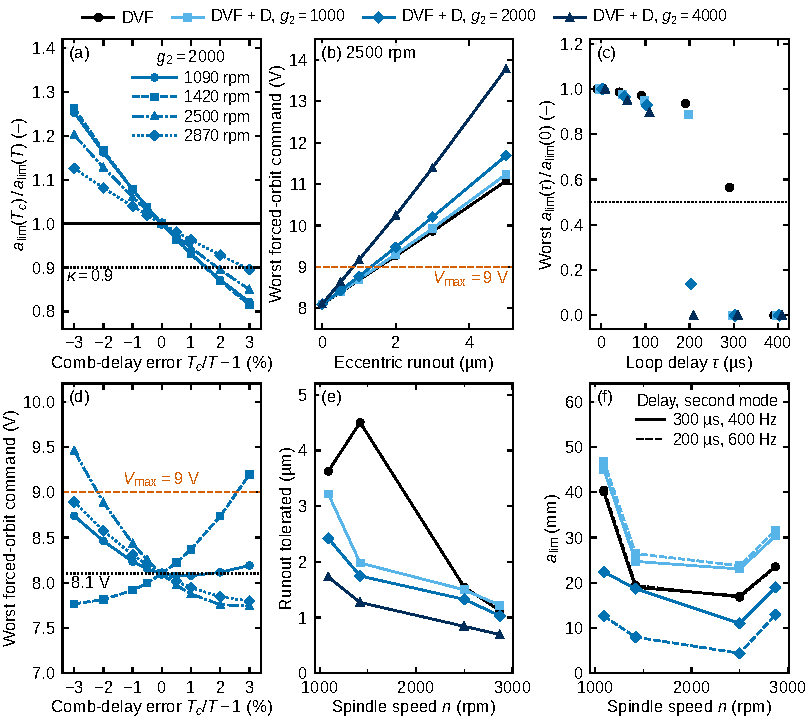
\includegraphics[width=\textwidth]{figures/fig10_robustness.pdf}
  \caption{Robustness of the delayed term (closed-form zero-order model; designs as in Table~\ref{tab:drobust}). (a)~Linear limit against the comb-delay error, relative to the exact delay ($g_2=\SI{2000}{\volt\second\per\metre}$), and (d)~worst forced-orbit command in the same cases. (b)~Worst forced-orbit command at \SI{2500}{\rpm} against the eccentric runout, and (e)~the runout at which it reaches \SI{9}{\volt}. (c)~$\alim(\tau)/\alim(0)$, worst over the four speeds and the three assumed second modes, at the computed delays only (0: loop unstable without cutting; dotted: 0.5; markers offset horizontally for legibility). (f)~$\alim$ of DVF and of DVF\,+\,D with $g_2=1000$ and 2000, with \SI{300}{\micro\second} and the \SI{400}{\hertz} mode (solid) or \SI{200}{\micro\second} and the \SI{600}{\hertz} mode (dashed); $g_2=4000$, unstable without cutting in both cases, is not shown.}
  \label{fig:robust}
\end{figure}


\subsection{Simulator build}\label{supp:delayed-sim}

A second build of the simulator of Section~\ref{app:simulator}, used only when a new option is requested, adds: $g_2$ and $k_d$, with $\dot x(t-T)$ from the derivative of the cubic Hermite interpolant of the stored history (zero before $t=0$); a comb delay $T_c=\rho T$ in place of $T$ in Eq.~\eqref{M-eq:comb-law}, for a speed error ($\rho\approx1$) or a spindle-period comb ($\rho=N_t$); an eccentric radial runout $r_j=r_0\cos(2\pi j/N_t+\theta_r)$ of tooth $j$, which adds $r_j-r_{j+k}$ (indices modulo $N_t$) to the chip cut against the pass $k$ tooth periods back, so that runout enters only the regenerated chip; and a loop delay $\tau$. The default build is bit-identical to that of Sections~\ref{M-sec:feasibility}--\ref{M-sec:certificates}.
% src: README §13.3 (identical preprocessed source and disassembly, fingerprint test); src/tdsim.c (COMB build), src/c4_robust.py (runout model); tests/test_c4_comb.py (test_comb_build_with_vanishing_gains_is_the_default, test_delayed_velocity_of_the_comb_term, test_loop_delay_uses_the_motion_one_delay_back, test_spindle_comb_vanishes_on_the_runout_orbit)

\subsection{Closed-form model and its verification}\label{supp:delayed-cf}

The zeros of $\Delta(s)$, Eq.~\eqref{eq:comb-char}, in $\operatorname{Re}s>0$ were counted by the argument principle along the imaginary axis up to \SI{5}{\kilo\hertz}, in steps of \SI{0.25}{\radian\per\second}. The limit is the first depth with such a zero, found by a scan in steps of \SI{3}{\percent} from \SI{0.3}{\milli\metre} and bisection; a design whose loop is unstable without cutting is given the limit 0. The forced orbit, spindle-periodic with runout, has the harmonics $X_k=G(ik\Omega)F_k/\Delta(ik\Omega)$, with $F_k$ from the static force of one slice over a revolution, integrated over the depth as in Eq.~\eqref{M-eq:Fm} with $mN_t$ replaced by $k$ (without runout, $F_{mN_t}=F_m$).

The closed-form limits agree with those of the collocation model within $2\times10^{-4}$ (four cases), and the simulated limits are 1.003--1.015 times the closed-form ones in seven cases that include the spindle-period comb, comb-delay errors of $\pm\SI{2}{\percent}$ and loop delays of 200--\SI{400}{\micro\second}. The settled command agrees within \SI{1.3}{\percent} in seven of eight cases with runout or delay errors, and differs by \SI{0.22}{\volt} in the eighth, where it is only about \SI{1}{\volt}. The assumed second modes were not checked in the simulator.
% src: src/c4_robust.py (delta, unstable_zeros: W_MAX = 2 pi x 5 kHz, DW = 0.25 rad/s; a_lim_cf: 0 if unstable at a = 1e-7 m, scan by 3 % from 0.3 mm, bisection; slice_force_revolution, orbit_command); tests/test_c4_comb.py (test_closed_form_limit_is_the_collocated_limit, 4 cases, rel 2e-4; test_comb_limit_matches_the_simulator, 3 cases, rel 1.5 %); results/c4_robust.npz, c4_summary.json (robust.td_limit_ratio 1.0025-1.0148, 7 cases; td_orbit_ratio 0.990-1.013 in 7 cases; 0.988 V against 0.767 V, i.e. 29 %, at 1090 rpm, 25 mm, spindle comb, 3 um runout); README §13.3, §13.10

\subsection{Proportional term}\label{supp:delayed-p}

For $g_1,g_2\ge0$, $\operatorname{Re}K(s)=g_1+g_2\bigl[1-e^{-T\operatorname{Re}s}\cos(T\operatorname{Im}s)\bigr]\ge g_1$ in $\operatorname{Re}s\ge0$, which gives property (ii) of Section~\ref{supp:delayed-prior}. The P term is not passive: the real part of $k_dE(i\omega)/(i\omega)$ is $k_d\sin(\omega T)/\omega$, which changes sign. Under the authority rule of Section~\ref{supp:delayed-limit} it shifts the linear limit by a nearly constant 2.9--\SI{3.0}{\milli\metre} ($k_d=\SI{-3e5}{\volt\per\metre}$) or 9.7--\SI{9.9}{\milli\metre} ($k_d=\SI{-e6}{\volt\per\metre}$) at every speed, about \SI{1}{\milli\metre} per \SI{-e5}{\volt\per\metre} as property (iii) of Section~\ref{supp:delayed-prior} predicts (with $g_1=1500$ at \SI{2500}{\rpm}, $k_d=\SI{-e5}{\volt\per\metre}$ raises the limit by \SI{0.98}{\milli\metre}), so that its relative gain is largest where the DVF limit is small (Table~\ref{tab:supp-dlim-p}).
% src: results/c4_limits.npz (feas_a_lim differences, recomputed: p3e5 - dvf 2.89-3.02 mm, p1e6 - dvf 9.66-9.93 mm); results/c4_summary.json (limits.feasible.p3e5, p1e6); README §13.5; tests/test_c4_comb.py (test_negative_kd_opposes_regeneration: +0.98 mm for kd = -1e5 V/m at 2500 rpm, g1 = 1500)

\begin{table}[!htbp]
  \centering
  \caption{Linear stability limit of the DVF\,+\,P designs ($g_2=0$) over 251 speeds under the authority rule of Table~\ref{tab:dlim}, which they complete; $k_d$ in \si{\volt\per\metre}.}
  \label{tab:supp-dlim-p}
  \small
  \begin{tabular}{@{}lccc@{}}
    \toprule
    Design & $\alim$ (\si{\milli\metre}) & Ratio to DVF & Median ratio\\
     & & median (range) & authority / bound\\
    \midrule
    DVF\,+\,P, $k_d=-3\times10^5$ & 16.9--45.7 & 1.12 (1.07--1.21) & 1.13 / 1.09\\
    DVF\,+\,P, $k_d=-10^6$ & 23.8--52.7 & 1.40 (1.23--1.70) & 1.45 / 1.29\\
    \bottomrule
  \end{tabular}
\end{table}
% src: results/c4_summary.json (limits.feasible.p3e5, p1e6: a_lim_mm 16.91-45.71 and 23.80-52.65, ratio_to_dvf, ratio_authority_limited, ratio_gain_bounded); README §13.5

\subsection{Further details: design rule, entries and gain map}\label{supp:delayed-details}

The design's own limit in the authority rule is the first unstable depth of the collocation model, found by an upward scan and bisection, as stability need not be monotone in the depth. The DVF gain is limited by authority at \SIrange{1060}{3000}{\rpm}. Adding $g_2$ or $k_d$ changes $g_1$ by at most \SI{9.7}{\volt\second\per\metre}, because the forced demand peaks below $0.9\alim$ of either design. With the gain bound lifted to \SI{20000}{\volt\second\per\metre} at the 56 speeds where DVF sits on it, the DVF gain rises to 3010--\SI{8760}{\volt\second\per\metre}, and DVF\,+\,D ($g_2=2000$), whose $\lvert K\rvert$ peaks at $g_1+2g_2$, reaches 1.31--1.68 times the DVF limit.
% src: src/c4_comb.py (a_lim_ctrl, feasible_g1); results/c4_limits.npz (max |g1 - g1_DVF| = 9.7 V s/m); results/c4_summary.json (limits.uncapped.dvf_g1 3008-8761 V s/m; d2000/DVF 1.31-1.68); results/c4_limits.npz (feas_g1: DVF below 3000 at 195 speeds, 1060-3000 rpm); README §13.4

In the entry simulations the depth ladder was scaled to each design's own $\alim$. The face-entry limit is 14.1--\SI{40.6}{\milli\metre} for DVF and 29.5--\SI{60.8}{\milli\metre} with D; DVF reaches at least $0.97\alim$, and with D it stays at 0.85--$0.98\alim$ at 600, 1000, 1200, 1300, 2300, 2400 and 2800--\SI{3000}{\rpm}. The step-entry limit is 12.9--\SI{28.2}{\milli\metre} for DVF and 12.7--\SI{35.1}{\milli\metre} with D; D raises it by up to 1.27 times at \SI{1900}{\rpm} and lowers it by up to \SI{0.2}{\milli\metre} at \SIrange{2700}{3000}{\rpm}. At \SIrange{600}{1300}{\rpm} the larger DVF gain of this rule (2480--\SI{3000}{\volt\second\per\metre}) itself raises the step-entry limit 1.05--1.34 times above that at $g=1500$ (Section~\ref{M-sec:bistab-map}). Near the forced resonance (\SI{2000}{\rpm}) the face entry with the gain of Section~\ref{M-sec:feasibility} and $g_2=2000$ reached the top of the depth ladder, $1.05\alim$, whereas runs of 2000 revolutions start to chatter at $0.9996\alim$: the 300-revolution classifier biases such near-limit boundaries high (Section~\ref{M-sec:bistab-prot}).
% src: results/c4_entry.npz (designs feas_dvf, feas_d2000: a_entry, a_lim, g1; face entry with D below 0.98 a_lim at 600, 1000, 1200, 1300, 2300, 2400, 2800-3000 rpm), results/c4_summary.json (entry: step_clip and edge_clip mm; edge_clip.paper+2000: max 1.05); results/c4_summary.json (entry: edge_clip feas_dvf over_a_lim min 0.974); results/c1_map.npz (a_step_clip at g = 1500 compared at the eight speeds 600-1300 rpm: ratios 1.05-1.34, recomputed; DVF g1 2481-3000 V s/m there); verification/tdsim/check10_forced_resonance_long_runs.json (c4_face_entry: 2000 rpm, g1 = 250.9, g2 = 2000, td300 1.05, onset 0.9996); README §13.6

The certified gain map used the default solver settings, as for the surface of Section~\ref{M-sec:cert-c2}, and its certificates were rescaled to the rigorous bound $\bar b$ as in Section~\ref{M-sec:cert-lmi}, by factors of 0.59--1, below 0.99 only where $u_0$ almost vanishes. Of the 1360 delayed candidates (four speeds, 17 depths, 20 pairs), 913 were certified, 270 were linearly unstable, 169 had a saturated forced orbit and 8 had no candidate that passed the check; of the 1768 DVF candidates (26 gains), 835, 722, 207 and 4. The certificate-optimal DVF gain rises with the depth from 500 to 2200--\SI{2700}{\volt\second\per\metre}. At 24--\SI{26}{\milli\metre}, about twice the axial pitch, the forced command is small (2.5--\SI{3.8}{\volt} for the DVF optimum), DVF is certified again, and the best delayed design has $g_1=1500$--2000 with $g_2=500$--1000. A kick of \SI{1}{\milli\metre\per\second} carries 0.2--\SI{0.6}{\percent} of the cutting impulse of one tooth period at \SI{34}{\milli\metre}.
% src: src/c4_comb.py (run_gainmap, FAST settings); results/c4_gainmap.npz (delayed: 913 of 1360 certified, 270 unstable, 169 orbit saturates, 8 without a passing candidate; DVF: 835 of 1768, 722, 207, 4; maximising designs per speed and depth; DVF optimum b_max 2.5-3.8 V at 24-26 mm); results/c3_summary.json (errata.c4_gainmap: size_factor 0.593-1); paper/figures/figure_numbers.json (fig09.gainmap_factor); impulse share recomputed from Eq. (impulse) with src/params.py: 0.22-0.59 % at 34 mm; README §13.7, §14.9

\subsection{Further details of the validation}\label{supp:delayed-valid}

The certificates of the 100 validation points used strict solver settings and the check of Section~\ref{M-sec:cert-check}. At 11 points, at 6 and \SI{10}{\milli\metre} at \SI{1420}{\rpm} and at \SI{6}{\milli\metre} at \SI{2870}{\rpm}, no kick up to \SI{3}{\metre\per\second} ended in chatter. At the eight deepest points (30 and \SI{34}{\milli\metre}, $g_2$ up to 4000) $\Delta v^*$ exceeds the certificate 2.1--3.7 times. The 32 map designs also received the off-axis test of Section~\ref{M-sec:cert-c2}, and none of the 2304 runs ended in chatter; in the sampled check of the collocation model, $\mathcal V$ stayed at or below 0.998, which is only a consistency check.
% src: results/c4_validate.npz, results/c4_validate2.npz (unsettled 0; td_min infinite at 11 points; offaxis 0/1728 and 0/576; proof_vmax 0.998); results/c3_summary.json (errata.c4_validate: deep 2.08-3.69); src/c4_comb.py (run_validate, run_validate2: TIGHT settings); README §13.8, §14.9

At the 22 pairs the map design reaches 0.82--3.02 times $\Delta v^*$ of the 26-gain DVF, 0.81--3.02 times that of the better DVF design, and 0.99--3.02 times (median 1.19) at \SI{18}{\milli\metre} and deeper. The six same-$g_1$ pairs where the DVF certificate is at most \SI{2.1}{\milli\metre\per\second} are 1420 and \SI{2870}{\rpm} at 18 and \SI{22}{\milli\metre}, \SI{2500}{\rpm} at \SI{22}{\milli\metre} and \SI{1090}{\rpm} at \SI{34}{\milli\metre}; the next pair (\SI{1090}{\rpm}, \SI{30}{\milli\metre}, DVF certificate \SI{2.6}{\milli\metre\per\second}) gives 1.45. The same-$g_1$ design raises $\Delta v^*$ from 4.0 to \SI{10.4}{\milli\metre\per\second} at \SI{1420}{\rpm} and \SI{18}{\milli\metre}. Freeing authority can add to the basin: at \SI{2500}{\rpm} and \SI{22}{\milli\metre} the map design ($g_1=500$, forced command \SI{2.5}{\volt} instead of \SI{7.7}{\volt}) reaches 7.8 against \SI{5.4}{\milli\metre\per\second} for the same-$g_1$ design. The preference of the certificate for a small $g_1$ can also narrow the basin: at \SI{1420}{\rpm} and \SI{14}{\milli\metre} the map design reaches 17.9 against \SI{21.8}{\milli\metre\per\second} for DVF.
% src: results/c4_summary.json (validate2: comb_over_dvf 0.82-3.02; comb_over_better_dvf 0.81-3.02; pairs_mmps: 1420 rpm, 18 mm: 4.02 -> 10.42 mm/s; 2500 rpm, 22 mm: 7.78 and 5.38 mm/s; 1420 rpm, 14 mm: 17.91 and 21.76 mm/s); against the better DVF at >= 18 mm: 0.99-3.02, median 1.19, recomputed from pairs_mmps; same_g1_near_dvf_limit (6 pairs) and next pair 1090 rpm, 30 mm: 1.45; results/c4_gainmap.npz (2500 rpm, 22 mm: b_max 2.46 V at g1 = 500 and 7.68 V at g1 = 1900); README §13.8

\subsection{Further details of the robustness study}\label{supp:delayed-robust}

The robustness designs have $g_1=1400$--\SI{2540}{\volt\second\per\metre}, equal across $g_2$ within \SI{1.1}{\volt\second\per\metre}. The runout tolerance was found by linear interpolation of the largest forced command, over 40 depths up to $0.9\alim$ and eight runout phases, between the computed runouts of 0, 0.5, 1, 2, 3 and \SI{5}{\micro\metre}. It falls monotonically with $g_2$ except from DVF to $g_2=1000$ at \SI{2870}{\rpm} (1.12 and \SI{1.22}{\micro\metre}).
% src: src/c4_robust.py (designs, GUARD = 0.9; RUNOUT grid and linear interpolation of the 9 V crossing; worst_orbit_command: N_DEPTH = 40, n_psi = 8); results/c4_robust.npz (g1 1395.8-2539.5 V s/m); results/c4_summary.json (robust.by_rpm.runout_tolerance_um); README §13.9

\paragraph{Comb-delay error} For $g_2=2000$ the limit stays within 0.93--1.08 of its nominal value at $\pm\SI{1}{\percent}$. An error of $-\SI{2}{\percent}$ raises the limit by 8--\SI{17}{\percent} and one of $+\SI{2}{\percent}$ lowers it by 7--\SI{13}{\percent}. At $\pm\SI{3}{\percent}$ the forced command exceeds \SI{9}{\volt} in two of the eight cases (\SI{2500}{\rpm} at $-\SI{3}{\percent}$, \SI{1420}{\rpm} at $+\SI{3}{\percent}$), and with $g_2=4000$ already at $\pm\SI{2}{\percent}$ in three of the eight. In the simulator, the face entry at \SI{2500}{\rpm} follows the shifted limit within \SI{0.1}{\percent}, from 36.2 to \SI{28.7}{\milli\metre} as the error goes from $-2$ to $+\SI{2}{\percent}$.
% src: results/c4_summary.json (robust.by_rpm, tooth comb: eps_a_lim_mm, relative 1.081-1.166 at -2 % and 0.869-0.928 at +2 %; eps_worst_cmd_V: 9.20 V at 1420 rpm, +3 %, 9.45 V at 2500 rpm, -3 %; tooth comb 4000 above 9 V at 1420 rpm +2 %, 2500 and 2870 rpm -2 %; td_face_eps: 28.74/28.77 to 36.22/36.25 mm); paper/figures/figure_numbers.json (fig10: eps_pm1_rel 0.93-1.08, eps_minus2_rel 1.08-1.17, eps_pm3_cases_above_9V 2 of 8); README §13.9, §13.10

\paragraph{Loop delay and assumed modes} With the identified mode alone and \SI{400}{\micro\second}, DVF\,+\,D with $g_2=2000$ keeps 24.0--\SI{35.8}{\milli\metre} against 17.3--\SI{31.7}{\milli\metre} for DVF. With the \SI{400}{\hertz} mode and a delay of \SI{300}{\micro\second} its limit is 11.0--\SI{22.4}{\milli\metre}, against 17.1--\SI{40.1}{\milli\metre} for DVF. With the \SI{600}{\hertz} mode and a delay of \SI{200}{\micro\second} the limit of $g_2=2000$ collapses to 4.4--\SI{12.9}{\milli\metre}, whereas the design with $g_2=1000$ keeps 23.7--\SI{46.8}{\milli\metre}, against 16.8--\SI{40.4}{\milli\metre} for DVF. DVF itself collapses at \SI{400}{\micro\second} with the 600 and \SI{800}{\hertz} modes. At \SI{2500}{\rpm}, \SI{300}{\micro\second} and the \SI{400}{\hertz} mode the critical root of DVF\,+\,D ($g_2=2000$) lies near \SI{473}{\hertz}, where $\lvert K\rvert=\SI{2861}{\volt\second\per\metre}$ is about half its peak $g_1+2g_2=\SI{5396}{\volt\second\per\metre}$ but the phase of $K$ ($K=g_1+g_2E$), $-\ang{36}$, adds to the lag of the delay.
% src: results/c4_summary.json (robust.by_rpm tau_a_lim_mm: one mode at 400 us 24.04-35.77 against 17.29-31.68 mm; mode_400Hz at 300 us 10.99-22.37 against 17.06-40.06 mm; mode_600Hz at 200 us, g2 = 2000 4.41-12.92 mm, g2 = 1000 23.74-46.84 mm against DVF 16.79-40.44 mm; DVF at 400 us: 0 with 600 Hz, 0-1.83 mm with 800 Hz); README §13.9 (473 Hz, |K| = 2861 V s/m, -36 deg: README only; consistent with |K(i 2 pi f)| = 2898-2860 V s/m at -36.0 deg for f = 473.0-473.5 Hz, g1 = 1395.8)

\paragraph{Spindle-period comb} With $T_c=N_tT$ the comb vanishes on the runout orbit and tolerates runout like DVF (1.12--\SI{4.46}{\micro\metre}), but it is no remedy: without delay its limit is close to that of DVF ($+0.3$ to $+\SI{4}{\percent}$; $+\SI{27}{\percent}$ at \SI{2500}{\rpm}), and it is very sensitive to phase (at \SI{2500}{\rpm} the limit jumps from 20 to \SI{80}{\milli\metre} with \SI{100}{\micro\second} of delay) and to speed errors (9.7--\SI{13.6}{\volt} of forced command at $-\SI{2}{\percent}$).
% src: results/c4_summary.json (robust.by_rpm spindle comb: a_lim 39.18/20.08/20.16/22.89 mm against DVF 37.64/19.40/15.91/22.82 mm; runout_tolerance_um 1.12-4.46; 2500 rpm, one mode: 20.16 -> 80.24 mm at 100 us; eps_worst_cmd_V 9.74-13.62 V at -2 %); README §13.9
